\section{Design}
\label{sec:design}

Named after the analogous technique in chess artificial intelligence \cite{iterative-deepening-chess-ai},
Iterative Deepening
%likewise
makes progressively deeper searches of the state space until the CPU budget is exhausted.
In this context, the depth is the number of PPs used.
Hence, our tool \quicksand~schedules multiple MC instances in parallel to simultaneously test many different subsets of the available PPs.
We refer to each unique set of PPs as a {\em job},
and prioritize them based on number of PPs, ETA, and whether they include data-race PPs,
We rely on state-space estimation \cite{estimation}
to predict which jobs are likely to complete within a reasonable time,
before actually testing a large fraction of interleavings for each.
The overall goal is to decide automatically when to defer testing a state space,
so an inexpert user can provide only their total CPU budget as a test parameter,
and to enable completing appropriately-sized jobs within that budget.
We seek to maximize completed state spaces,
as each one serves as a guarantee that all interleavings possible with its PPs were tested.

Note that Iterative Deepening is a {\em wrapper} algorithm around stateless MC.
A MC tool is still used to test each state space, and other reduction techniques are still applicable.
Moreover, because Iterative Deepening treats the set of preemption points as mutable,
it can add new preemption points reactively based on any runtime analysis.
We focus on run-time data-race detection~\cite{hybriddatarace,tsan,ifrit} as the mechanism for finding new preemption candidates.

%%%%%%%%%%%%%%%%%%%%%%%%%%%%%%%%%%%%%%%%%%%%%%%%%%%%%%%%%%%%%%%%%%%%%%%%%%%%%%%%

\subsection{Initial PP configuration}
\label{sec:initial-pp}

Iterative Deepening must be seeded with a set of initial state spaces,
which can be any number of subsets of the statically-available PPs SSS-MC would use.
For completeness (\sect{\ref{sec:totalverif}}), the maximal state space must be included among these.

For testing user-space code, we begin with the four PP sets from Figure~\ref{fig:id}:
$\{yield\}$,
$\{yield,lock\}$,
$\{yield,unlock\}$,
and $\{yield,lock,unlock\}$,
By extension, these also introduce PPs on any other primitives
which use
internal locks,
such as condvars or semaphores.
Preempting on voluntary switches such as {\tt yield} is always necessary to maintain the invariant that only one thread runs between consecutive PPs.
%so the {\tt yield} PP is always implicitly enabled.

For kernel-level testing, we consider interrupt-disabling analogous to locking,
so we also preempt just before a disable-interrupt opcode ({\tt cli}) and just after interrupts are re-enabled ({\tt sti})\footnote{
%(to appropriate the names of the x86 instructions)
During data-race detection, {\tt cli}/{\tt sti} are treated as a single global lock.
%as {\tt cli}'d memory accesses can still race with others that have interrupts on.
Some kernels disable preemption without disabling interrupts,
which can be communicated to the MC using manual annotations. %of that API.
This also assumes uni-processor scheduling; for SMP kernels, replace {\tt cli}/{\tt sti} with spinlocks.}.
\quicksand~is configured to begin with
$\{yield\}$,
$\{yield,lock\}$,
$\{yield,unlock\}$,
$\{yield,cli\}$,
$\{yield,sti\}$,
and $\{yield,lock,$ $unlock,cli,sti\}$.
As a heuristic, we don't test every intermediate subset such as $\{lock,sti\}$,
which could potentially be improved in future work (\sect{\ref{sec:future}}).

%%%%%%%%%%%%%%%%%%%%%%%%%%%%%%%%%%%%%%%%%%%%%%%%%%%%%%%%%%%%%%%%%%%%%%%%%%%%%%%%

\subsection{Choosing the best job}

\newcommand\PendingJobs{\ensuremath{\mathcal{P}}}
\newcommand\SuspendedJobs{\ensuremath{\mathcal{S}}}
\newcommand\GetETA[1]{ETA(#1)}
\newcommand\GetPPSet[1]{PPSet(#1)}
With a limited CPU budget, we must avoid running tests that are likely to be fruitless.
Hence, we separate the available PP sets into a set of {\em suspended} jobs (partially-explored state spaces with high ETAs),
and a set of {\em pending} jobs (untested ones with unknown ETAs).
When the MC reports an ETA too high for some job,
we compare with other pending and suspended jobs to find another one more likely to complete in time.
%
Our method for doing so, listed in Algorithm~\ref{alg:shouldworkblock}, is the heart of Iterative Deepening.
%\footnote{
%Though its worst-case performance is $O(mn)$ in the
%%number of pending and suspended jobs,
%sizes of $\mathcal{P}$ and $\mathcal{S}$,
%in practice the non-constant portion beyond line 4 runs very infrequently
%and is negligible compared to the exponentially-sized state spaces.}.
Its main feature is understanding that if \GetPPSet{$j_1$} $\subset$ \GetPPSet{$j_2$},
and $j_1$ is suspended,
then $j_2$'s state space is guaranteed to be strictly larger, so $j_2$ will take at least as long.
Hence we should avoid testing $j_2$ unless $j_1$ is later resumed and its ETA improves after further execution. %over time.
%reveals that it might finish in time after all.
Similarly, whenever a job finds a bug, we cancel all pending superset jobs, as they would find the same bug.

\begin{algorithm}[t]
	\SetKwInOut{Input}{Input}
	%\textbf{Function} GetBestJob($j_0$, PendingJobs, SuspendedJobs): \\
	\Input{$j_0$, the currently-running job}
	%\Input{$eta$, $j_0$'s predicted completion time}
	\Input{\PendingJobs, the list of pending jobs, sorted by decreasing heuristic priority}
	\Input{\SuspendedJobs, the list of already-suspended jobs, sorted by increasing ETA}
	\If{\GetETA{$j_0$} $<$ HeuristicETAFactor $\times$ TimeLeft()}{
		return $j_0$ // Common case: job is expected to finish.
	}
	\ForEach{job $j_P \in$ \PendingJobs}{
		// Don't run a pending job if a subset of it is already suspended; its ETA would be at least as bad. \\
		\If {$\forall j_S \in$ \SuspendedJobs, \GetPPSet{$j_S$} $\not\subset$ \GetPPSet{$j_P$}}{
			return $j_P$
		}
	}
	%// no pending jobs; maybe resume a suspended job \\
	\ForEach{job $j_S \in$ \SuspendedJobs}{
		\If{\GetPPSet{$j_0$} $\not\subset$ \GetPPSet{$j_S$}
			$\land$
			\GetETA{$j_0$} $>$ \GetETA{$j_S$}}{
			// If a subset of $j_S$ is also suspended, don't run the larger one first. \\
			\If{$\forall j_{S2} \in$ \SuspendedJobs, \GetPPSet{$j_{S2}$} $\not\subset$ \GetPPSet{$j_S$}}{
				return $j_S$
			}
		}
	}
	return $j_0$ // \GetETA{$j_0$} was bad, but no other $j$ was better.
	\caption{Suspending exploration of a state space in favour of a potentially smaller one.}
	\label{alg:shouldworkblock}
\end{algorithm}

%
We also account for the inherent inaccuracy of ETA estimates.
Line 1 heuristically scales up the time remaining to avoid suspending jobs too aggressively
in case their ETAs are actually overestimated.
Lines 12-14 account for the
%bizarre
possibility that among two suspended jobs,
%given two jobs,
%%$j_1,j_2$,
\GetPPSet{$j_1$} $\subset$ \GetPPSet{$j_2$}
but
\GetETA{$j_1$} $>$ \GetETA{$j_2$}.
This can arise because estimates tend to get more accurate over time,
and $j_1$ perhaps ran much longer before suspending.
% In such scenarios,
We heuristically assume the smaller job's ETA is more accurate
to avoid repeatedly resuming larger jobs briefly while their ETAs only become worse
(it lets us avoid thrashing in \quicksand).

%%%%%%%%%%%%%%%%%%%%%%%%%%%%%%%%%%%%%%%%%%%%%%%%%%%%%%%%%%%%%%%%%%%%%%%%%%%%%%%%

\subsection{Data-race preemption points}
\label{sec:classifying}

During stateless MC, runtime data-race detection may find data-race candidates that we wish to investigate further.
Because data races indicate access pairs that can interleave at instruction granularity,
it is logical to re-execute the test and issue preemptions just before those instructions to test alternate thread interleavings~\cite{racefuzzer,portend}.

\newcommand\AllJobs{\ensuremath{\mathcal{J}}}
\begin{algorithm}[t]
	\SetKwInOut{Input}{Input}
	\Input{$j_0$, the currently-running job}
	\Input{\AllJobs, the set of all existing (or completed) jobs}
	\Input{$\alpha$, an instruction reported by the MC as part of a racing access pair}
	\If{$\forall j \in \AllJobs,$
	\GetPPSet{$j_0$} $\cup$ $\alpha$
	$\not\subseteq$
	\GetPPSet{$j$}
	}{
		AddNewJob(\GetPPSet{$j_0$} $\cup$ $\alpha$, HeuristicPriority($\alpha$)) \\
	}
	\If{$\forall j \in \AllJobs,$ \GetPPSet{$j$} $\neq \{yield, \alpha\}$}{
		AddNewJob($\{yield, \alpha\}$, HeuristicPriority($\alpha$))
	}
	\caption{Adding new jobs with data-race PPs.}
	\label{alg:handledatarace}
\end{algorithm}

With Iterative Deepening, this is a simple matter of creating a new state space with an additional PP enabled on the racing instructions by each thread, as shown in Algorithm~\ref{alg:handledatarace}.
We call these {\em data-race PPs}.
Note that even though a data race may involve two different instructions, $\alpha$ and $\beta$, we add new state spaces with only one new PP at a time.
Rather than adding a single large state space, %configured to preempt on both involved instructions,
i.e., $AB =$ \GetPPSet{$j_0$} $\cup$ $\alpha$ $\cup$ $\beta$,
we prefer to add multiple smaller jobs which have a higher chance of completing in time, i.e.,
$A =$ \GetPPSet{$j_0$} $\cup$ $\alpha$ and
$B =$ \GetPPSet{$j_0$} $\cup$ $\beta$.
If $A$ and $B$ are bug-free, they will in turn add $AB$ later.
The condition on line 1 ensures that we avoid duplicating any state spaces with multiple data-race PPs;
for example, $AB$ is reachable by multiple paths through its different subsets, but should be added only once.

Furthermore, we do not always strictly increase the number of PPs when we find a new data race.
For each instruction involved in a data race, \quicksand~adds two new jobs:
a ``small'' job to preempt on that instruction only (line 5),
and a ``big'' job to preempt on that instruction as well as each PP used by the reporting job (line 2).
%
Hence,
%together with the logic in \sect{\ref{sec:classifying}},
each {\em pair} of racing accesses will spawn four new jobs, as shown in Figure~\ref{fig:new-dr-jobs}.
%
The rationale of spawning multiple jobs is that we don't know in advance which will be most fruitful:
while the big job risks not completing in time,
the small job risks missing the data race entirely if the original PPs were required to expose it.
% TODO CAMREADY: Put numbers here.
In practice, we observed some bugs found quickly by these small jobs, and other bugs missed by the small jobs found eventually by the big jobs.
This phenomenon motivates Iterative Deepening to prioritize the jobs at run-time.

\begin{figure}[t]
	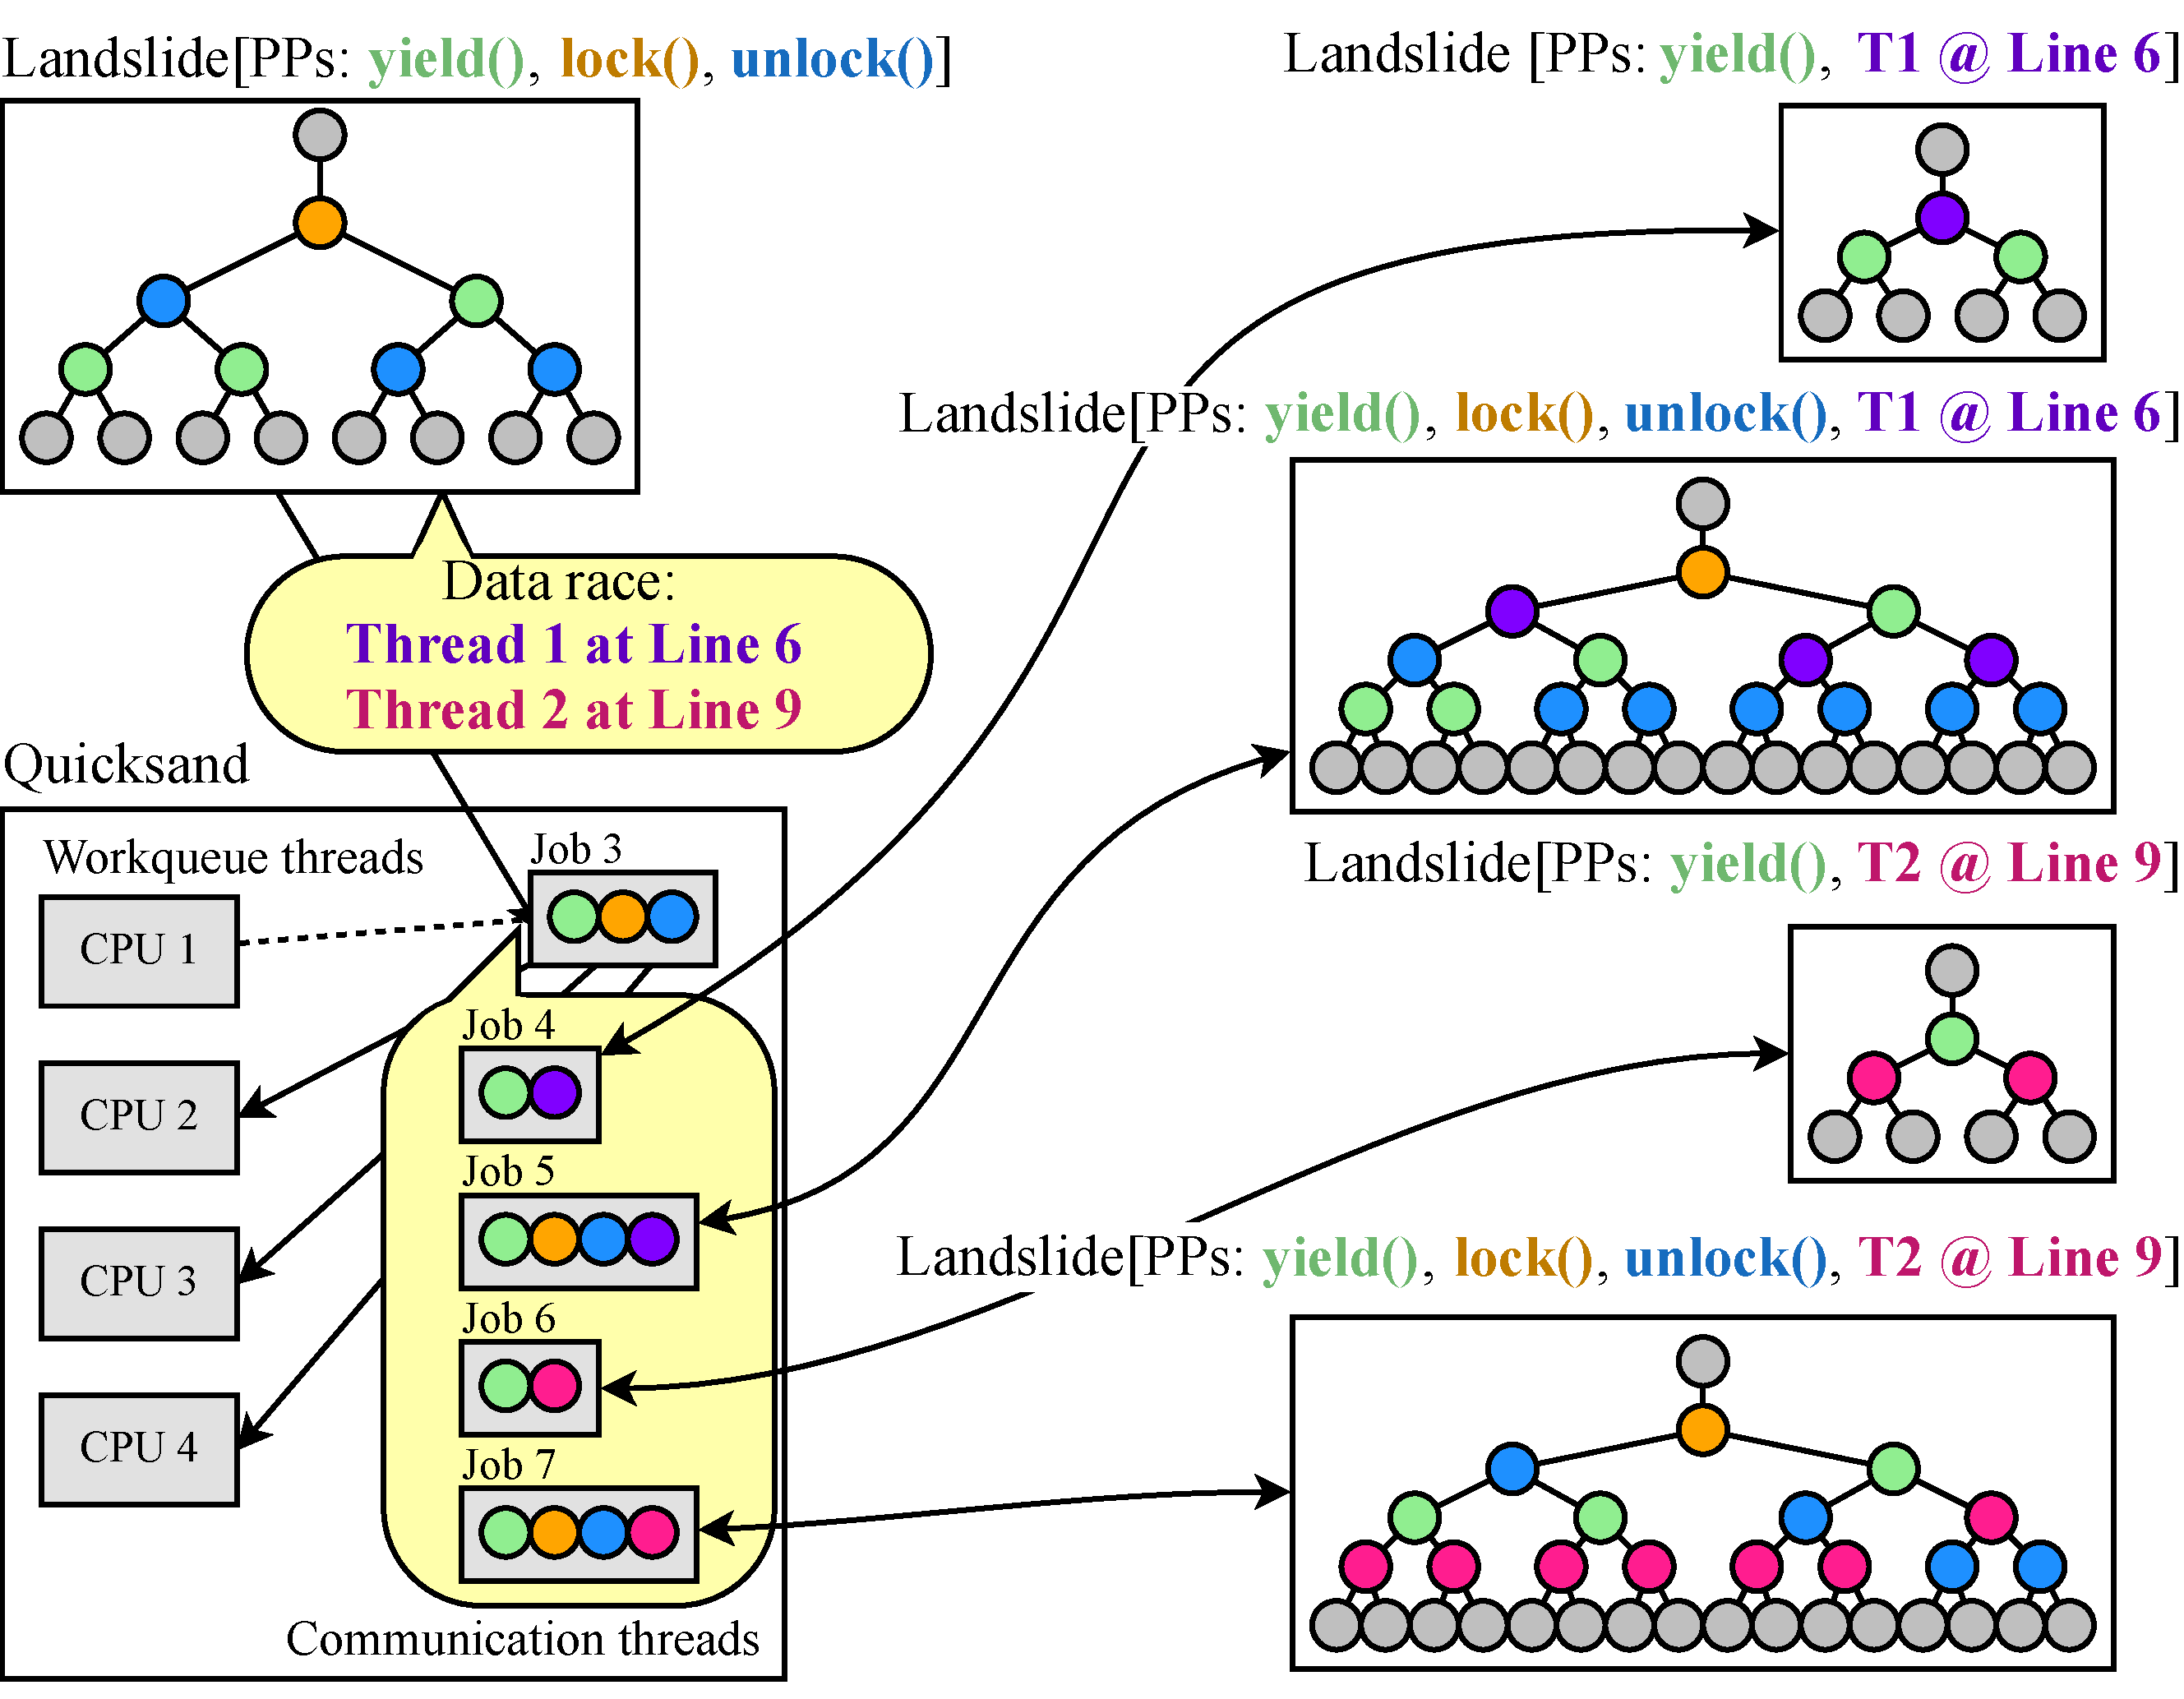
\includegraphics[width=0.48\textwidth]{dr-jobs-v2.pdf}
	\caption{\quicksand~manages the exploration of multiple state spaces, communicating with each MC instance to receive ETAs, data race candidates, and bug reports.
		When an access pair is reported as a data race candidate, we generate a new PP for each access, and add new jobs corresponding to different combinations of those with the existing PPs.}
	\label{fig:new-dr-jobs}
\end{figure}

The new state spaces may expose a failure, in which case we report a data-race bug,
or complete successfully, indicating a benign or false-positive data race.
They may also uncover a new data-race candidate entirely, %in some alternate interleaving,
in which case we may iteratively advance to a superset state space containing PPs for both racing access pairs.
Being constrained by a CPU budget,
we may time out before completing a data race's associated state space,
in which case we report a potential false positive that the user must handle (\sect{\ref{sec:future}}).

%When \landslide~detects a data race, it reports each of the two memory accesses involved in the race.
%Each report indicates the program counter value (PC) associated with the access, as well as some further conditions to help filter away unrelated executions of the same instruction on different data.
%(For example, many parts of a codebase might call {\tt list\_insert()}, but only one callsite does so without adequate locking.)
%Ideally, the PC would be qualified by a full backtrace, but tracing the stack is too expensive to do for each shared memory access.
%Instead, \landslide~qualifies the PC with
%(a) the current thread ID and
%% FIXME: We don't actually do this.
%(b) the most recent {\tt call} instruction.
%% (a crude approximation of a stack trace)
%% which are much cheaper, as we carry them around all the time already
%Note that we do {\em not} qualify data races by the shared memory address,
%which can change based on different interleavings of previous code
%(for example, depending on the result of {\tt malloc()}).
%% especially when malloc is involved.
%%Figure~\ref{fig:dont-filter-dr-by-address} shows example code where qualifying by memory address will miss the bug.

%%%%%%%%%%%%%%%%%%%%%%%%%%%%%%%%%%%%%%%%%%%%%%%%%%%%%%%%%%%%%%%%%%%%%%%%%%%%%%%%

\subsection{Heuristics}
% List of all heuristix:
% HOMESTRETCH - last 60sec of test, don't suspend
% ETA_THRESH - "to let its ETA stabilize"
% eta factor
% shold_reproduce -- small dr jobs are not allowed to add further instances of themself (why not? don't remember)
% priority change between suspected and confirmed dr
Algorithm~\ref{alg:shouldworkblock} allows heuristically scaling a job's ETA when comparing to the time budget,
to express how pessimistic we are about the estimate's accuracy.
We use a scaling factor defaulting to 2 based on the results in \cite{estimation}.
%though we allow changing it via the command line.
We also include a heuristic to
%ignore ETAs entirely
never suspend jobs before they pass a certain threshold of interleavings tested,
with a default of 32,
so that their ETAs have some time to stabilize.

We classify data-race candidates as {\em single-order} or {\em both-order} \cite{portend}
based on whether the MC observed the racing instructions ordered one or both ways in the original state space,
Single-order candidates are more likely to be false positives (\sect{\ref{sec:overview-dr}}),
although preempting during the access itself is necessary to say for sure.
Hence, we add PPs for both types of candiates, and heuristically prioritize jobs with both-order data-race PPs
(indicated by the HeuristicPriority($\alpha$) call in Algorithm~\ref{alg:handledatarace}).
For single-order races, we do not initially add a PP for the later access at all:
if preempting on the first access can reorder the race, it will be upgraded to both-order in the new state space, and we will add the second PP then.
%should it be needed, preempting on the first access will suffice to upgrade the race to both-order.
